\documentclass[tikz]{standalone}
\usepackage{pgfplots}
\pgfplotsset{compat=1.15}
\usepackage{mathrsfs}
\usetikzlibrary{arrows,calc}
\usepackage{tkz-euclide}
\pagestyle{empty}

\definecolor{AngleClr}{rgb}{0,0.39215686274509803,0}
\definecolor{ShapeClr}{rgb}{0.6,0.2,0}

\begin{document}

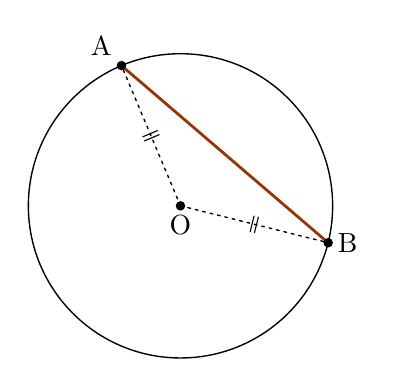
\begin{tikzpicture}[scale=.75]
\tkzSetUpLine[line width=1pt,color=black]
\tkzSetUpPoint[fill=black]

\tkzDefPoints{0/0/B,1.5/3/A,5/0/C}

\tkzDefCircle[circum](A,B,C) \tkzGetPoint{O}

\tkzDrawCircles[line width=0.5pt,color=black](O,A)

\tkzDrawSegments[line width=0.5pt,color=black,dashed,dash pattern=on 1pt off 1.75pt](O,A O,C)

\tkzDrawPolygon[color=ShapeClr](A,C)
\tkzDrawPoints[size=3](A,C,O)

\tkzLabelPoint[above left](A){$\rm A$}
\tkzLabelPoint[right](C){$\rm B$}
\tkzLabelPoint[below](O){$\rm O$}

\tkzMarkSegments[mark=||,size=3](O,A O,C)

\end{tikzpicture}
\end{document}

